\documentclass[conference]{IEEEtran}
\IEEEoverridecommandlockouts
\usepackage{cite}
\usepackage{amsmath,amssymb,amsfonts}
\usepackage{algorithmic}
\usepackage{graphicx}
\usepackage{textcomp}
\usepackage{xcolor}
\usepackage{url}
\usepackage{wrapfig}
\usepackage{float}
\usepackage{lscape}
\usepackage{longtable}
\usepackage{booktabs}
\def\BibTeX{{\rm B\kern-.05em{\sc i\kern-.025em b}\kern-.08em
    T\kern-.1667em\lower.7ex\hbox{E}\kern-.125emX}}
\begin{document}

\title{ESCAPE Y2K - An Integrated Escape Room}

\author{Kyle L. Sedgwick, Jake D. Bales, Nami Eskandarian}

\author{\IEEEauthorblockN{1\textsuperscript{st} Kyle L. Sedgwick}
    \IEEEauthorblockA{\textit{College of Engineering} \\
        \textit{University of Utah}\\
        Salt Lake City, U.S \\}
    \and
    \IEEEauthorblockN{2\textsuperscript{nd} Jake D. Bales}
    \IEEEauthorblockA{\textit{College of Engineering} \\
        \textit{University of Utah}\\
        Salt Lake City, U.S \\}
    \and
    \IEEEauthorblockN{3\textsuperscript{rd} Nami Eskandarian}
    \IEEEauthorblockA{\textit{College of Engineering} \\
        \textit{University of Utah}\\
        Salt Lake City, U.S \\}
}



\maketitle

\begin{abstract}
    “ESCAPE Y2K” is an interactive escape room experience that relies on computer
    engineering as its main control source. The escape room is built to be an autonomous,
    immersive, sci-fi, horror experience using digital/analog circuit design, image/audio
    processing, communication protocols, and embedded computing. Players
    will interact and solve puzzles under a time limit while avoiding fictional threats within
    the game in order to complete the experience and win. This is done with a time travel mechanic
    that allows players to forward or reverse an artificial clock that changes the time within
    the room and activates certain events that could both benefit and disadvantage them.
\end{abstract}

\begin{IEEEkeywords}
    Analog, Embedded Systems, Escape Room, Horror, Interactive, Networking, Science Fiction
\end{IEEEkeywords}

\section{Introduction}
Escape rooms are a fun and engaging way to promote critical thinking and puzzle solving for children and adults
alike. In most established escape rooms, there is a level of behind the scenes interaction with a room operator,
triggering events and unlocking clues as the players progress. This usually works quite well and allows for some
additional variability if the operator is given some creative freedom with how they run the escape room. However,
it also has an inherited limitation with requiring an operator for the room to function. For our capstone senior
project, we will create an autonomous escape room experience with multiple puzzles and random clue selection to
operate with some level of variance without the requirement of an external human operator.
\\
\indent In general, innovation in the escape room industry is minimal; if you've been to one or two you've seen how
pretty much any of them are going to work. The level of difficulty from room to room may vary, and some of the
puzzles could be interesting, but there haven't been any groundbreaking changes made to the scene since its inception.
Our goal is to create a system and design philosophy that will allow for a more streamlined and easily modifiable
design process for making more complex and dynamic escape rooms. We will accomplish this with custom analog and digital
systems, as well as a variable program to be executed on a central microcontroller to drive the escape room's
interactive elements.
\\
\indent The theming of Escape Y2K is an time-traveling analog horror experience. The story and aesthetics of the room
will be inspired by the public panic spurred from the unknown consequences to possibly occur as digital system
clocks update their year count to '00', and the ambiguity between it's interpretation as '2000' (Y2K) or '1900'.
The room will incorporate 'time-traveling' elements to play into this ambiguity and assume that a total system
failure would happen in all digital systems when the game clock strikes 12:00 AM on the turn of the century.

\section{Our Vision}
Our vision for this project is to take a unique spin on the formula that is most commonly used in escape rooms.
Instead of using a large amount of analog puzzles and a ``host'' that is in charge of controlling which parts of
the room are locked and unlocked when players complete certain actions, the room will adapt and progress on its
own as players advance through the various puzzles.
\\
\indent One of the major themes of the escape room is time travel. The experience will run
on a physical game clock that ticks between 1:00 PM and 12:00 (midnight) where certain events are
dependent on the time. This can include cabinets opening during a specific time interval or
locks having different passcode combinations depending on the hour hand. Players in the
room are able to rewind or forward the time however they wish based on the minimum and
maximum the time can go. Past 8:00, the game will transition to a darker, nighttime mode where
more horror elements will come into play that can affect the game's timer. The maximum amount
of time players will have to escape will be 30 minutes (subject to change), however, it may speed up under
certain conditions and give players less time.

\subsection*{What is an Escape Room?}
Escape rooms provide participants with an interactive and exciting puzzle experience.
Players start by being ``locked'' in a room (for safety reasons, players are never really
locked inside) with a set of instructions that lead them through a series of puzzles. Some of
these puzzles are more traditional, such as solving a cypher or figuring out a combination for a lock,
while others make the players think a little bit deeper. Many of these puzzles are on the simple size in
an attempt to have a good balance of fun and difficulty. And, many of these rooms attempt to fit their
puzzles within a certain theme, such as escaping from an Egyptian tomb or trying to escape from the zombie
apcalypse~\cite{wikipediaEscapeRoom}.

\subsection*{History of Escape Rooms}
There are a variety of escape rooms all throughout Utah and in other parts of the world as well. The phenomenon
started between 1981 and 1984 with the introduction of TV game shows ``The Adventure Game'', ``The Crystal Maze'',
``Fort Boyard'', and ``Knightmare''~\cite{wikipediaEscapeRoom}. Other mediums, such as escape the room video games, were also gaining traction
during these years and after, and in 2003 the first prototype escape room was showcased at GenCon Indy by
an individual named Jeff Martin. 2007, however, was the first year when escape rooms really began to pick up speed
with the creation of Real Escape Game by Takao Kato in Kyoto, Japan~\cite{whatIsAnEscapeRoom}. The first commercially available escape rooms
began to show up in the United States around the years 2012-2014, and as of November 2019 there are over 50,000 escape
rooms worldwide~\cite{wikipediaEscapeRoom}.

\subsection*{Our Motive}
Although not the first idea for our senior project, we feel that an escape room checks all of the
boxes that we are hoping to fulfill with the project. Some of these requirements were that our project
have some sort of meaning or functional purpose, that our project be fun or interactive, and that
it be something that excited us as a group, not just as individuals. We originally thought of developing some
sort of art piece based in computer science, which would have been given meaning and have had some form of
interactability, but wouldn't have provided us with the level of fun we were hoping to achieve.
We also thought of a variety of different games we could create, however, nothing seemed to really interest
every member of the group. The escape room is something unique, interesting, interactive, and will hopefully
provide those that are able to play with a fun and memorable experience!

\subsection*{Player Motivation}
Many escape rooms use a type of ``Mission Video'' to explain what is going to happen in the escape room~\cite{whatIsAnEscapeRoom}.
For our escape room, we are going to use a tape player that gives the people in the room information about
the story and why they are in the room in the first place. This tape player will also have other uses, which are
explained in more detail in the section about all of the puzzles in the escape room.

\section{What Makes This Escape Room Unique?}
Because this escape room is being developed as a computer engineering senior project, it will have a distinct emphasis
on puzzles that involve embedded computing, giving our room a deeper sense of connection between the separate parts.
This means that we will be using technology as a central theme throughout the room to help convey the emotions that we
are hoping the players will feel and also make the puzzles more interesting.

\subsection*{The Story}
Our escape room will be inside the office of a computer engineer/scientist acutely aware of the existential threat
of a time traveling beast capable of destroying the world as we know it when the turn of the century occours on
new year's day 2000 (Y2K). At this time, the beast will gain access to our dimension through a software oversight
with how dates are stored in computer systems of the time. The correction to this global flaw rests in the office
the players find themselves in, and they must hurry to disseminate the correcting code before time runs out and the
beast escapes.

\subsection*{How Horror Plays a Role}
In life, horror is an incredibly good motivator. Imagine you are being hunted by some alien creature that is here to
destroy the world and the only way to escape is so solve a collection of puzzles; you would gladly partipate!
In our escape room, this exact situation is something that we will be utilizing to push players to solve the puzzles
as fast as possible.

\subsubsection*{The Monster}
Many horror experiences begin with a mysterious and dangerous monster that is on the hunt. Our room will feature such a monster
that will come out when specific events are triggered or when the player clock reaches a certain time.
If the monster is revealed to the players, this will activate an event which will
speed up the game timer which shortens the time it takes to complete the room. The monster is an
active threat that the players must watch out for to avoid losing precious time to
solve every puzzle.

\subsubsection*{CRT TVs}
An original idea for the escape room was to create some sort of false window box that mounts on
the wall or a TV with an image of ``outside world'', but the vision had to be adjusted a little bit for flexibility.
Now the idea is more in line with the idea of analog horror, as stationary CRT TVs
give players a glimpse into what is happening as Y2K approaches.

The main image that the tvs show is an animated version of the old Windows XP wallpaper (pictured below).
This image will slowly shift to a more unsettling, discolored version of the wallpaper as the player clock advances. If the
clock reaches midnight, the monster event will occur which speeds up the game timer. At any time if the players
choose to speed up or reverse time, the TVs will play an effect similar to fast forwarding or reversing a tape.
Using a microcontroller, multiple video files will be stocked and played on the TV depending on the state of the
game. The time position chosen for the video is also synced with the time on the clock.

\begin{figure}[ht]
    \centering
    
\includegraphics[width=0.90\columnwidth]{Images/tvcomparison.png}
    \caption{The image shown on the TVs. As time goes on in-game, the scenery
        gets a little more disturbing.}
\end{figure}

These TVs are also where the monster will appear to the players during the monster events. At certain moments
during the nighttime segment, a light will occasionally shine out of the television screen across the room. This light acts as
the ``vision'' of the monster, and if a player is caught in the light then the monster will appear for the players,
speeding up the game timer. During this monster event, time will stop and the players cannot change the
time until they exit the monster's field of vision. To detect players, a proposed idea is installing a camera
onto the TVs and using image processing to find players that are brightened by the light. There is also
the potential solution of requiring players wear a vest with a color that the monster detects. The microcontroller
will communicate with the central computer running the game to know what to play and notify if a player is detected.

\begin{figure}[ht]
    \centering
    
\includegraphics[width=0.90\columnwidth]{Images/tvsketch.png}
    \caption{TVs shine light that can reveal players to the monster.}
\end{figure}

\subsubsection*{Audio}
Audio is one of the most important elements of both horror experiences and enviornmental storytelling.
In this escape room, we will be making extensive use of hidden speakers, audio distortion, and mechanical
sound production to create a deep auditory experience for the players. Many sound effects and voices can
be stored on a micro SD card of a MP3 controller to be triggered during certain events, or make the
cassette player ``play itself'' when no tape is inserted (by hijacking the speaker wires). Auditory cues
will be implemented when unlocking different boxes using electromagnets, solenoids, or other mechanical
devices to make a directly more natural sound. We intend to keep the players engaged and ``on edge'' with
unexplained noises being a frequent occourence.

\subsection*{Decoration}
As previously mentioned, escape rooms are usually based around a theme that affects almost
every part of the room. These things include the tools that the players are given, another list item,
and especially how the room is designed. We have a few ideas for how we want our room to look, but
the portability aspect of our room may make intricate decorations difficult. However, we want to make
our escape room experience as multi-dimensional as possible.

%Kyle, not sure if this is where you wanna put the info about the room layout, but it wouldnt be the worst spot, at least :P
% I'll put it just before the puzzles, so we can get the full room before adding sub-images for key puzzle parts
%       - Kyle
\section{Initial Room Layout}
While many aspects of our escape room are likely to be somewhat modular, and able to be re-arranged quickly,
some puzzles and in-game events will demand certain elements of the room to be set up in specific locations relative
to each other. For example, the clock controls, game clock, and action clock should all be in close proximity to each
other for ease of access. The CRT TVs should be pointed across the audio cassette player to limit
access during certain events. Finally, props need to be kept in repeatable
locations or lock boxes for consistency in certain puzzles.
\\
\indent In the below diagrams, there are a few key elements to notice. The black boxes with white screens
represent the CRT TVs that have sensors and lights to trigger during in-game events. The
grey towers are filing cabinets, to play into the office aesthetic of the game. The light green slab on the
desks in the corner is where we will have the chessboard, and the yellow head represents one of the busts
that will be included in some puzzles. The center podium will hold the cassette player. Finally, the orange circle
is the time clock, and the nearby green box represents the clock controls.

\begin{figure}[ht]
    \centering
    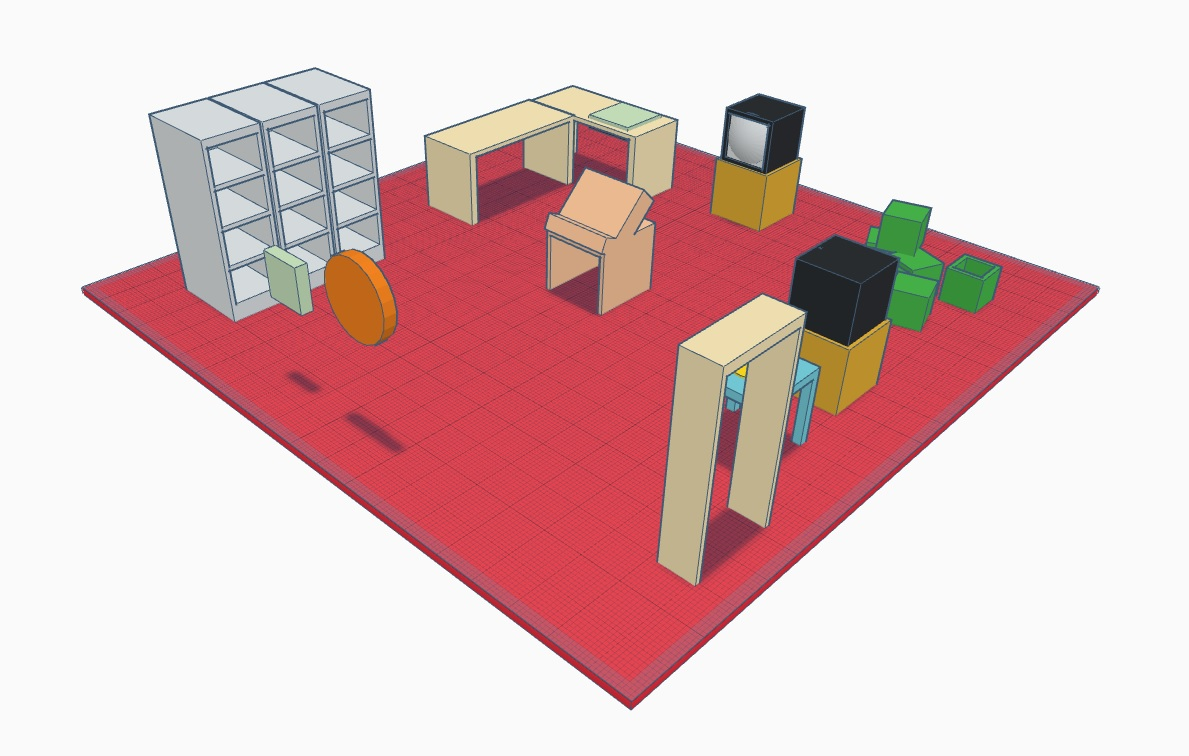
\includegraphics[width=0.90\columnwidth]{Images/EscapeRoomIsoFront.jpg}
    \caption{Front isometric scale depiction of the initial escape room layout.}
\end{figure}

\begin{figure}[ht]
    \centering
    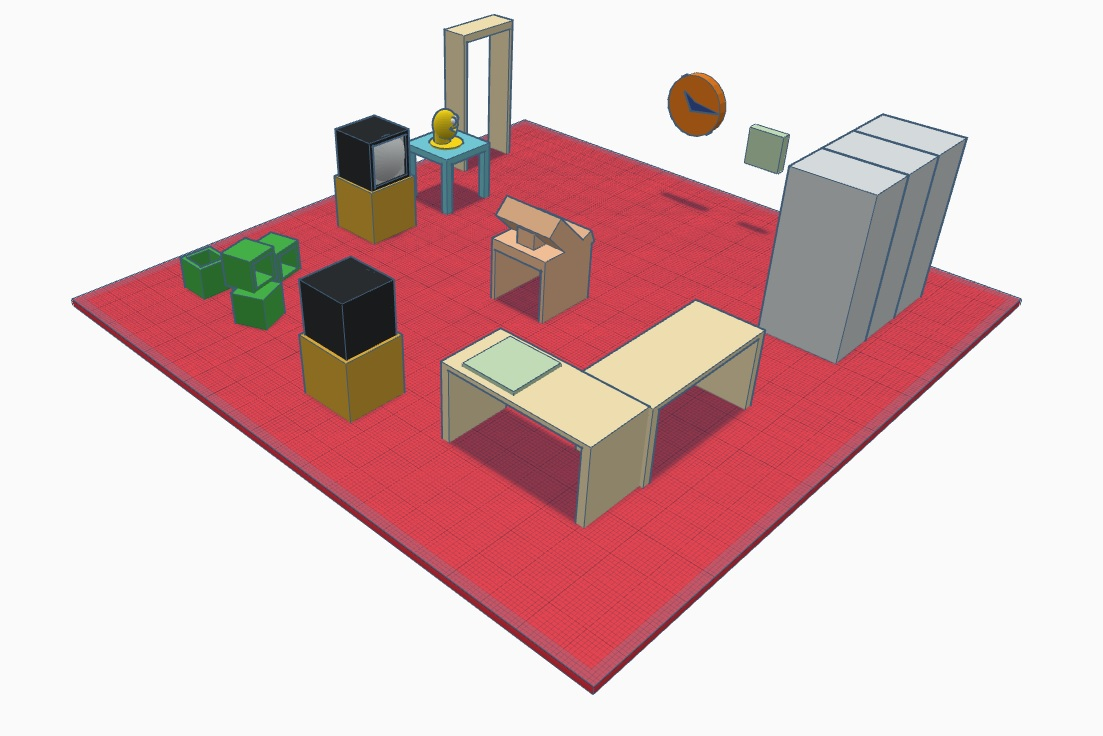
\includegraphics[width=0.75\columnwidth]{Images/EscapeRoomIsoRear.jpg}
    \caption{Rear isometric scale depiction of the initial escape room layout.}
\end{figure}


\section{Puzzles in our Escape Room}
This section contains a list of all of the puzzles that our escape room will feature, as well as
the solution to each of them. If you haven't already experienced the escape room, be warned that
this section does contain spoilers and will prevent you from experiencing the joy of solving the
puzzles on your own.
\\

% *************************************************************************************************************************************
% ************************************* THIS SECTION MUST BE REVISED ******************************************************************
% *************************************************************************************************************************************

\indent This section will be greatly expanded on as we decide what other puzzles we want to incorporate and how they will function.
A stretch goal we have is to have a pool of around 10-15 puzzles that can be randomly selected, so that each time a player is in the
room the experience will be different from the last. More may be added, depending on time contstraints and how many ideas we
have, but this is the idea for now.
\\
\indent Furthermore, we want to develop puzzles that take between 3-5 minutes to solve. This will be a hard balance
to achieve because we really want the puzzles to feel rewarding to solve, but also not frustrate the players
to a point when they are no longer able to continue with the escape room. Various tests will be run on friends, family members,
and anyone else who would like to help us tune the puzzles until they arrive at a happy medium.


\subsection{Chess Board Puzzle}
We have three ideas for the chess board puzzle. Two of the three ideas are based off the gold contact pins that are used
This puzzle will be one of the first things that players see, but also the last puzzle that they will solve.
Throughout the room and after solving various puzzles, players will receive chess pieces that, when
arranged in the correct format, will open the door that is keeping players in the room and stop the
catastrophic end of the world due to Y2K.

We have two ideas for the chess board puzzle. Both ideas are based off the gold contact pins that are used
to charge a pebble watch (and in other places in electronics as well). Basically, the idea
is to have these golden pins in each (or at least a lot) of the spaces of the chess board, with
a magnet underneath to help align the chess pieces when placed by the user. Only the pins that are used in
the solution would be wired up, decreasing the amount of soldering that would be required to make the chess
board and also leaving all of the other spaces as ``dummy'' spaces. The image below shows such a
mechanism, one that would be used for charging a smartwatch.

The third and final idea is to use magnetic switches underneath each of the places where we are wanting the players
to put the pieces. Each piece would have a magnet inside, and when they are all placed on the correct squares the
final door to the room would open. This solution is most assuredly easier since we are no longer able to identify
which piece is in a given square. However, if we are unable to figure out a good way to implement the previous
two solutions this is a definate option.

\begin{figure}[ht]
    \centering
    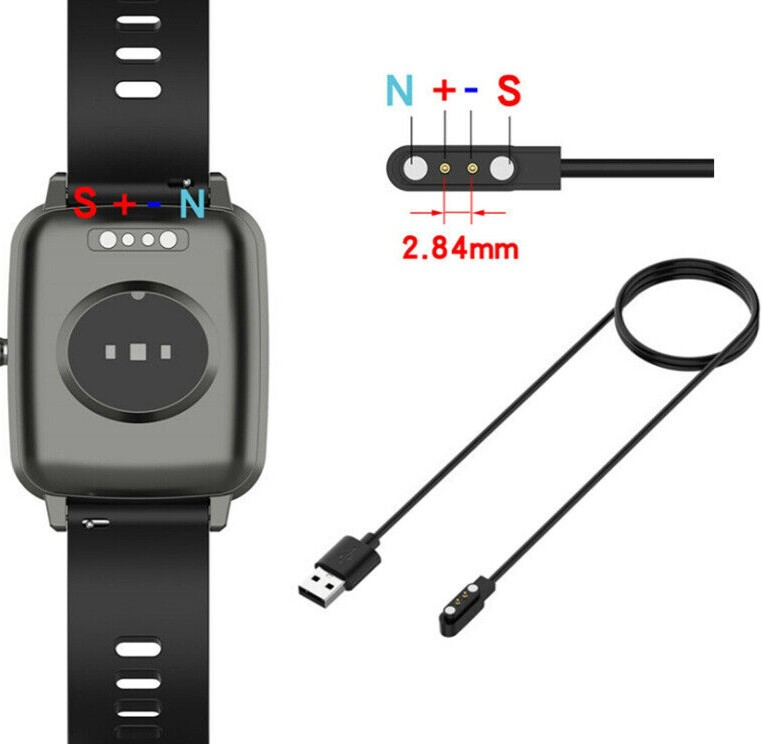
\includegraphics[width=0.75\columnwidth]{Images/pebble charger.jpg}
    \caption{Depiction of the contact pins that we plan on using for chess piece identification.}
\end{figure}

For our first idea, we are thinking of embedding resistors with different values into
each of the chess pieces. Then, if the chess piece is placed on a space that is wired for the solution,
the resistor value from that piece would be read and analyzed. If it is the correct value for that space,
part of the puzzle would unlock. And, if every piece is placed in the correct location, when a button is
pressed then the door to the room will open and the players will be able to escape! This will likely be done
by communicating to the central computer when the button is pressed whether the players
have successfully completed the puzzle or not.

The second idea is a bit less flushed out, however, the premise is the same. However, instead of using
a resistor to denote which piece is in which location, we would hook up some sort of tiny microcontroller that
has been programmed to, when powered on, just transmit its name over and over. This would allow a computer
to read the value that is being transmitted and determine if the piece has been placed in the correct location.


\subsection{Bust}
A small bust of a statue's head will be attached on a disc and situated
on a podium. This bust can be rotated physically, which will rotate the
disc under it as well. On the podium is a small hole that may contain a key
or chess piece. The disc will also have an indent on it. When the players
rotate the bust, if the disc is rotated so that the indent is overlapping
with the hole on the podium, the players are able to retrieve the key
or chess piece. As a bonus, the direction the bust is facing will be either
the lock the key unlocks or a clue as to where the chess piece goes.

\subsection{Tape Player}
An audio cassette player will be centered in the room, with one tape nearby
to be played as players first enter the room. The general function of the tape
player will be to both give the players story elements and instructions on
puzzles as they play, as well as be used to play clues or hints to the active
puzzle that the players are working on. Beyond these basic functions of the
cassette player, we will run wires from our microcontroller and digital audio
player into the built-in speaker of the cassette player to inject noises or music
files while the cassette player is not actively in use, or no tape is even in the
deck. This will add to the horror experience, and emulate rouge transmissions
being received over the duration of the escape experience.

\subsection{Encoded Audio/Radio Signal}
%KYLE, DONT FORGET TO TALK ABOUT YOUR SUPER DOPE ANALOG WAVE PUZZLE IDEA WITH PLAYING THE RIGHT CASSETTE TAPE
There are many devices available to convert an audio signal, supplied via an AUX audio cable
to a radio signal that can be transmitted via bluetooth or a similar radio protocol. One interesting
application of this intended to be implemented in this project is to either have a personal voice recorder
or audio cassette have a ``key'' encoded in the audio that will need to be transmitted to another
device in the room to unlock a lock box or clue. For example, a voice recorder may be found which has
a password spoken by a specific person's voice as a room access key. This recording will be played
to the correct access point to complete the puzzle and unlock the next item.

\subsection{Pressure Sensitive Chair}
Another idea that we have for a puzzle is something that requires every member of the escape room to participate.
Essentially, the idea is to have a number of chairs scattered throughout the room. Within each of these chairs
we will embed a pressure sensor that can detect when one of the players in the room has sat down in that chair.
Once every player in the room sits in the chairs that are scattered about, a lock of some sort will open and the
players will be able to progress!

In order to properly implement this puzzle we are going to need a few things. First of all, we are hoping that the
players will be able to move the chairs around the room freely, giving the illusion that they are just normal chairs.
This is going to require a small microcontroller to be hidden within the base of the chair that has Wi-Fi capabilities
(most likely the ESP 32 board, due to its small size and on-board Wi-Fi) and at least one GPIO pin to detect the change
in pressure when a player sits down on the chair. Furthermore, the board needs to have a relatively low power consumption
so that the chair battery doesn't die during the length of time the players will be in the escape room.

\subsection{All other puzzles...}
Currently, we have this limited number of planned puzzles, but more puzzles are expected to be added
as stretch goals. We plan on having this escape room experience last only between 20 to 30 minutes,
but this is a flexable duration that may change if time permits us to add a system that selects
only certain puzzles to be used in a given playthrough. This would allow for greater variability,
and for users to play the escape room more than once and solve different puzzles each time.
Once we have more base systems in place to make puzzles designing to be more streamlined, we can add
both to the number and complexity of puzzles.

\subsection*{Clock}
The clock that we have planned to use will be controlled through a single motor that turns the
dial used to set the clock (if you were planning on using it normally). We have already created
a mechanism that will control the clock and also allow others to control the clock as well. Under
no user input, the clock will function as normal, ticking forward at a constant rate of one hour per
minute. There are also two buttons, a fast-forward and a reverse button, that give players control
over the time that the clock is displaying. Once a button is pressed, a motor spins the clock
either forward or backwards, adjusting the events that are taking place in the room. An image of
the clock has been included below.

\begin{figure}[ht]
    \centering
    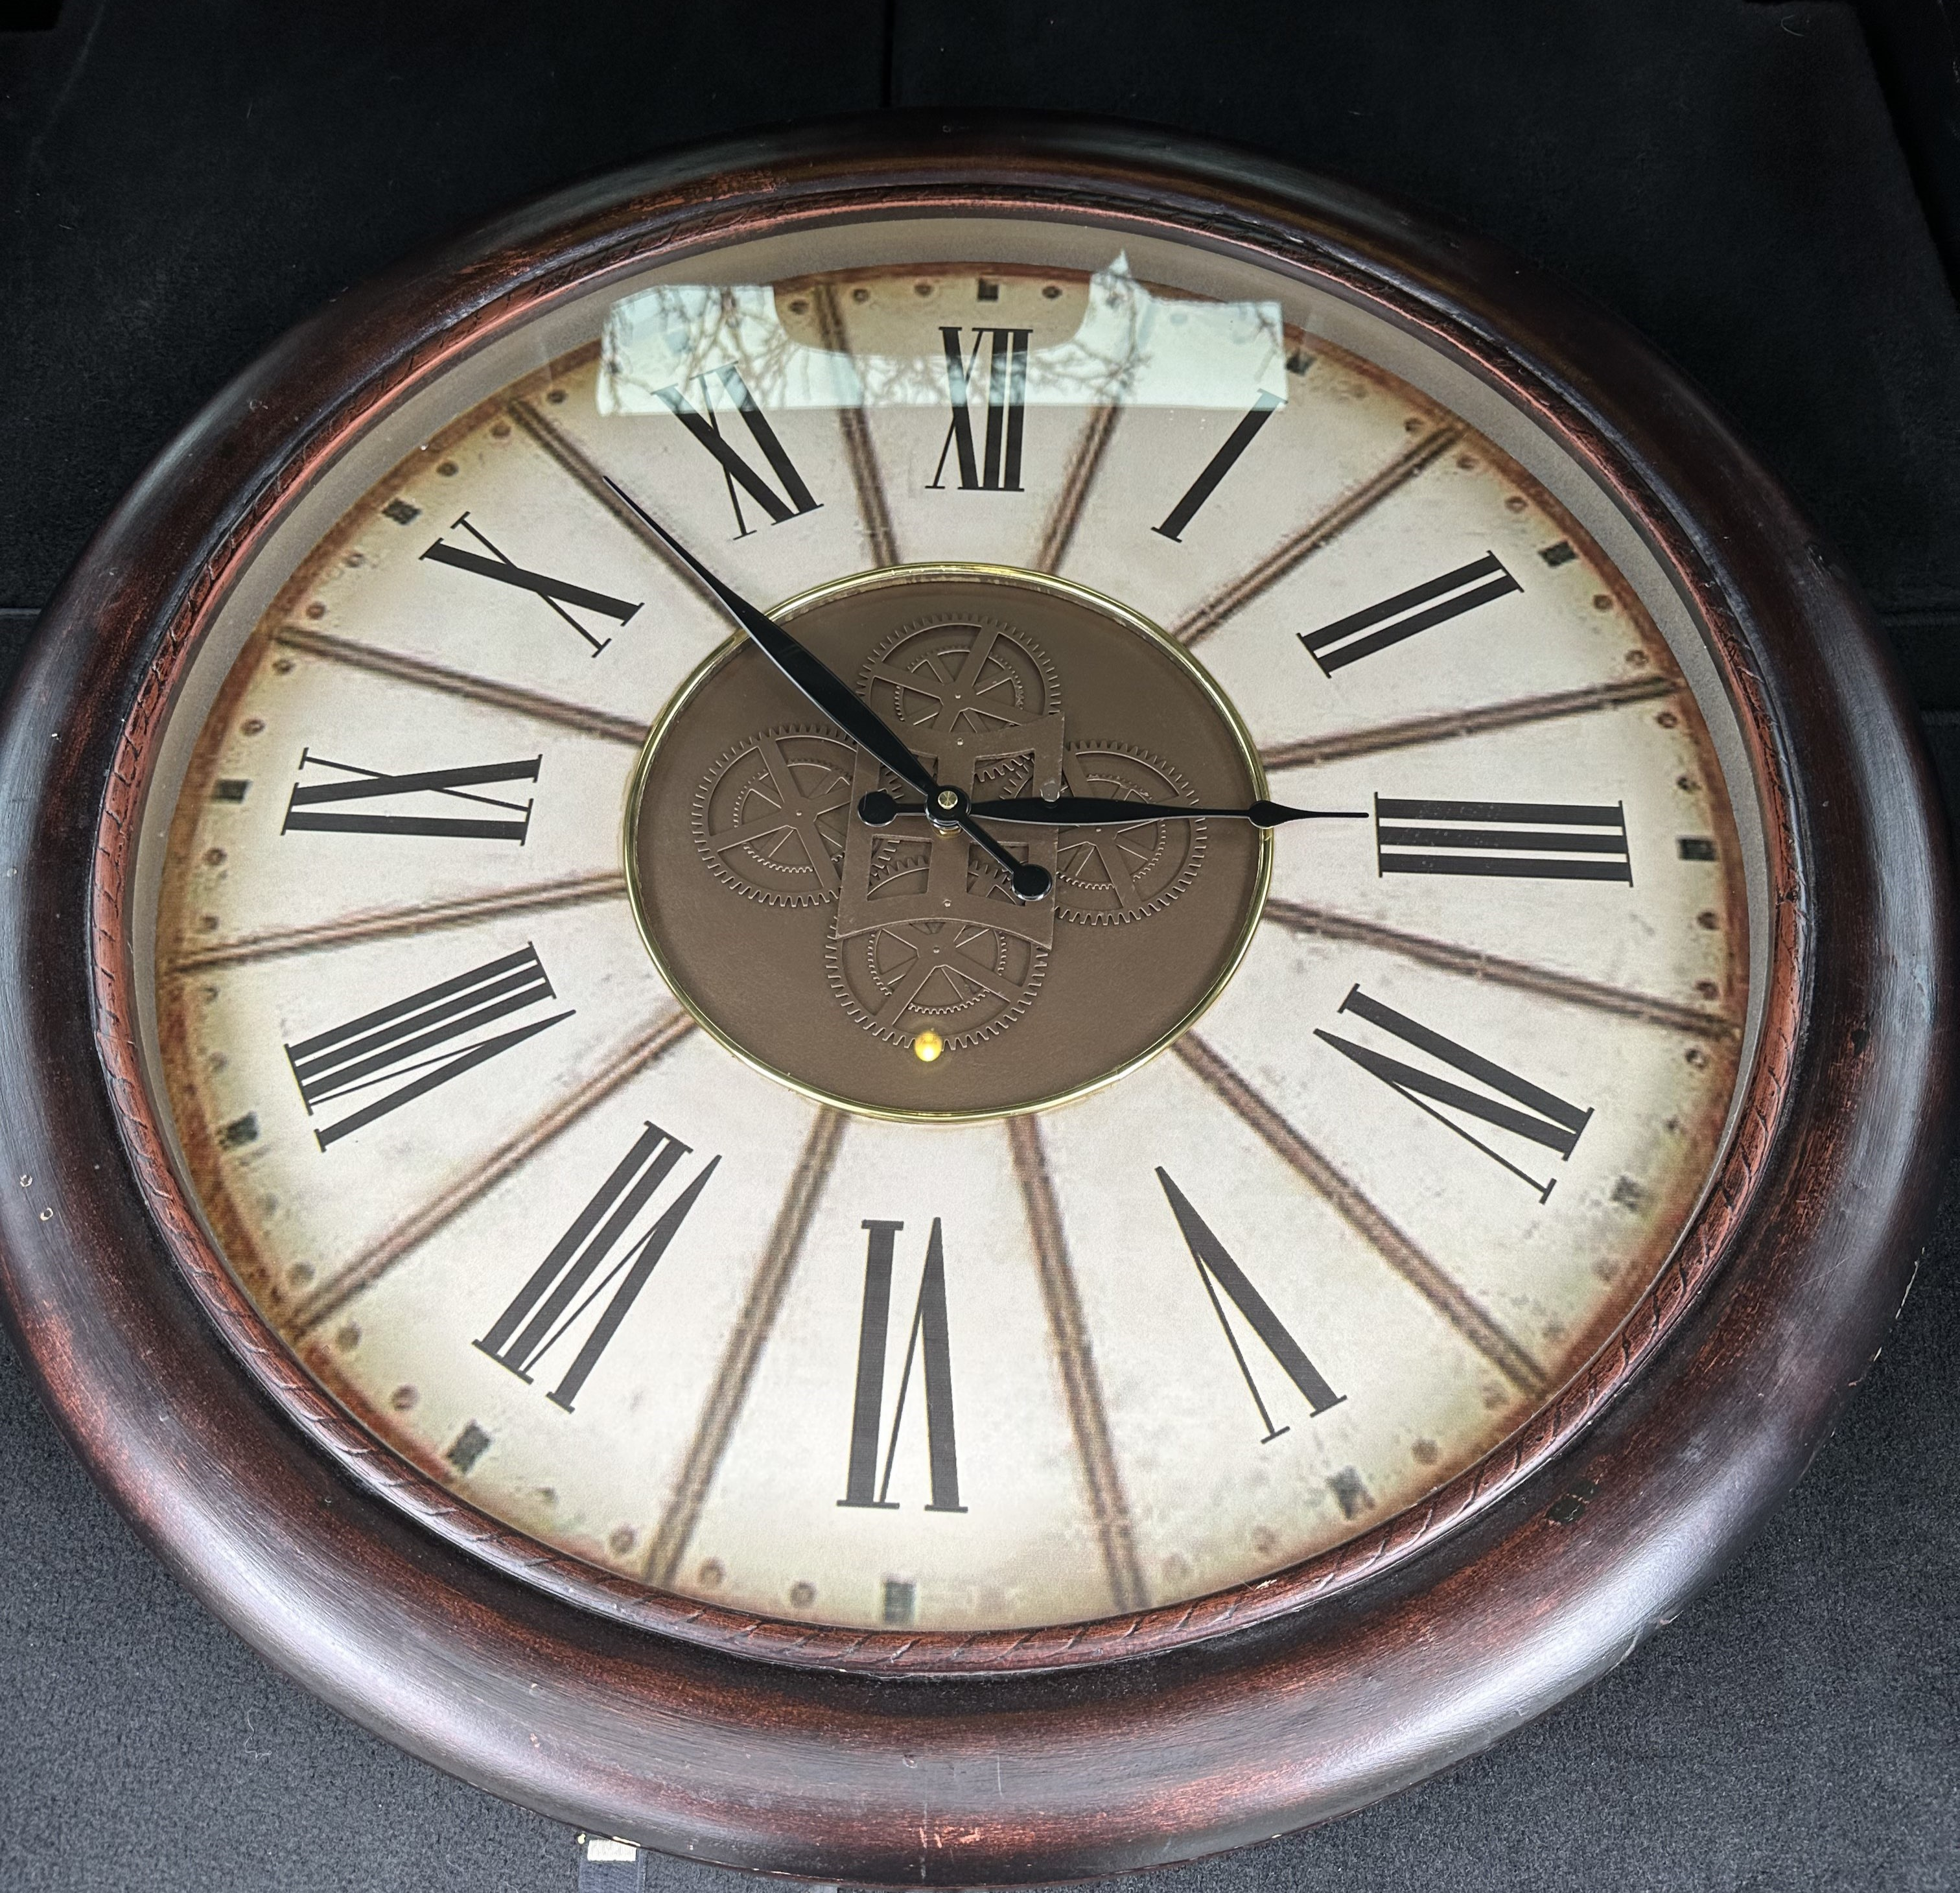
\includegraphics[width=0.85\columnwidth]{Images/big-clock.jpg}
    \caption{The big clock that we are using for the ``Player Clock''.}
\end{figure}

Our early prototype for this control is incredibly rough and does not use the microcontroller or the
motor that we are hoping to use in the final project, and is mostly just a proof of concept. In the
final project we are going to use a stepper motor that will allow us to have a much finer level of
control over what time the clock is displaying, and will also help the central computer keep track of
what time is being displayed. Furthermore, we are going to be 3D printing mounting brackets and other
components that will help the motor stay in place, rather than the mess of broken popsicle sticks and
duct tape that it currently is.

On top of the game clock is the game timer which will be displayed next to the door. This timer
shows the remaining amount of time left to complete the game and is visible at all times. When the
monster is revealed to the player during certain nighttime segments, the timer will go down at a
faster rate which will dissuade players from getting the monster's attention. Using an LED display,
the time will be outputted based on the value retrieved from the central computer's internal timer.

\section{Initial Mechanical Plans}
Traditional escape rooms use physical switches and locks to prevent access to certain information or
items until their related puzzles are completed or their key is found. Often, this takes the form of
traditional physical locks, with either combinations or keys. For the players to find the combination,
there is a puzzle with the correct combination embedded within it, or the combination is hidden in some
other form of media. Physical keys can be simply hidden arround the room, or be teased to the players
to hint at what puzzle must be completed to gain access to the physical key (like using magnets to move
the key out of a hole). While we will incorporate these traditional lock methods in our escape room,
we will also try to use more novel methods of controlling player access to resources via computer controlled
elements.

\subsection{Electromagnetic Locks}
Because many of our puzzles will include some form of electronic elements, it will be easy to add a
electromagnetic locking system that holds a door or drawer closed while the electromagnet is powered,
and at the completion of a puzzle, the magnet is turned off to grant access to the contents within the
container. While this can be a simple solution to controlling player access to key materials or information,
it may not be clear for players to identify what container has just become unlocked. An auditory cue may
be heard when the magnet deactivates, but if there are other sounds when this happens, it can be difficult
to identify where in the room the magnet has turned off.

\subsection{NFC/RFID}
Another electrical access control system is near-field communication and radio frequency identification
systems. These are often used for apartment and hotel access systems, and use either a keycard or
fob with an internal inductive circuit to open doors. We could make use of a similar system to control
access to certain areas of our escape room, but as this would require more specialized and expensive
equipment, we will only use this if a later-designed puzzle would benefit greatly from its implementation.

\subsection{Self-opening Motorized Latch Control}
In order to take advantage of the more unique control elements available to us by using computer
systems to control an autonomous escape room, we have devised a custom access control system that
will hold a container securely closed when locked, and open entirely on its own when unlocked. It
will include a system consisting of either stepper motors or servo motors, and a solenoid. If the container
includes a hinge, it will only require one motor and solenoid, but if the lid will remove entirely,
it will need at least two motors.
\\

\begin{figure}[ht]
    \centering
    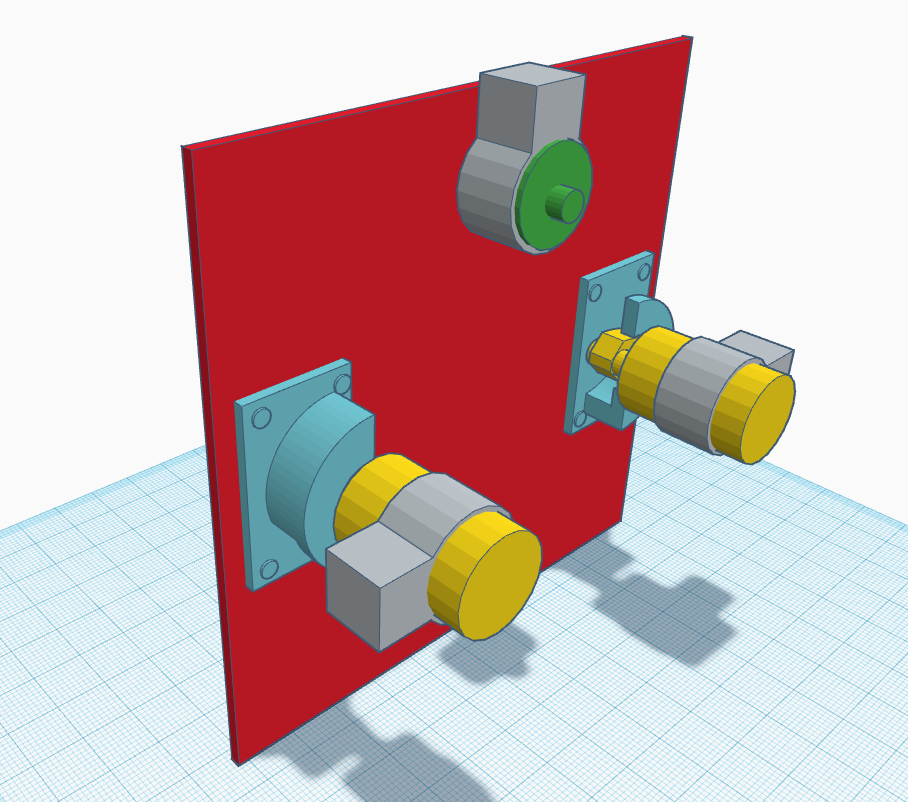
\includegraphics[width=0.85\columnwidth]{Images/LockMech.png}
    \caption{A custom locking system. The yellow objects are motors with a metal arm, and the green object is a solenoid.}
\end{figure}

\indent The motor(s) will have a metal arm attached to the motor shaft. This arm will rest between the
door or lid of the container, and a metal plate attached to the inside of the door or lid when locked.
This metal plate will only cover one half of the motor's movable range, and when the container is ``unlocked'',
the motor will rotate its metal arm out from under this plate, allowing the door or lid to be freely moved.
At this point, an active extruding solenoid will quickly activate and hit the door or lid of a container, to
open it without the player needing to do so manually. This will remove any ambiguity about what container
was just unlocked, so the players can quickly collect their earned materials and continue with the escape room
experience.

\begin{figure}[H]
    \centering
    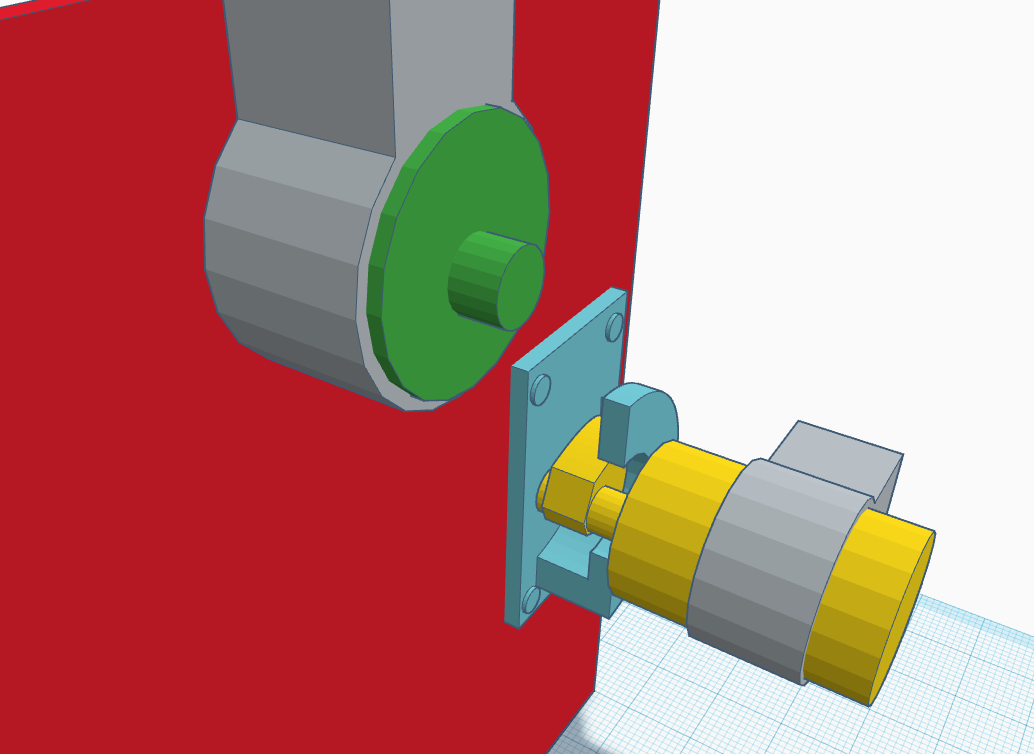
\includegraphics[width=0.85\columnwidth]{Images/ClosedLock.png}
    \caption{When the motor arms are under the metal plate, the container remains locked}
\end{figure}

\begin{figure}[H]
    \centering
    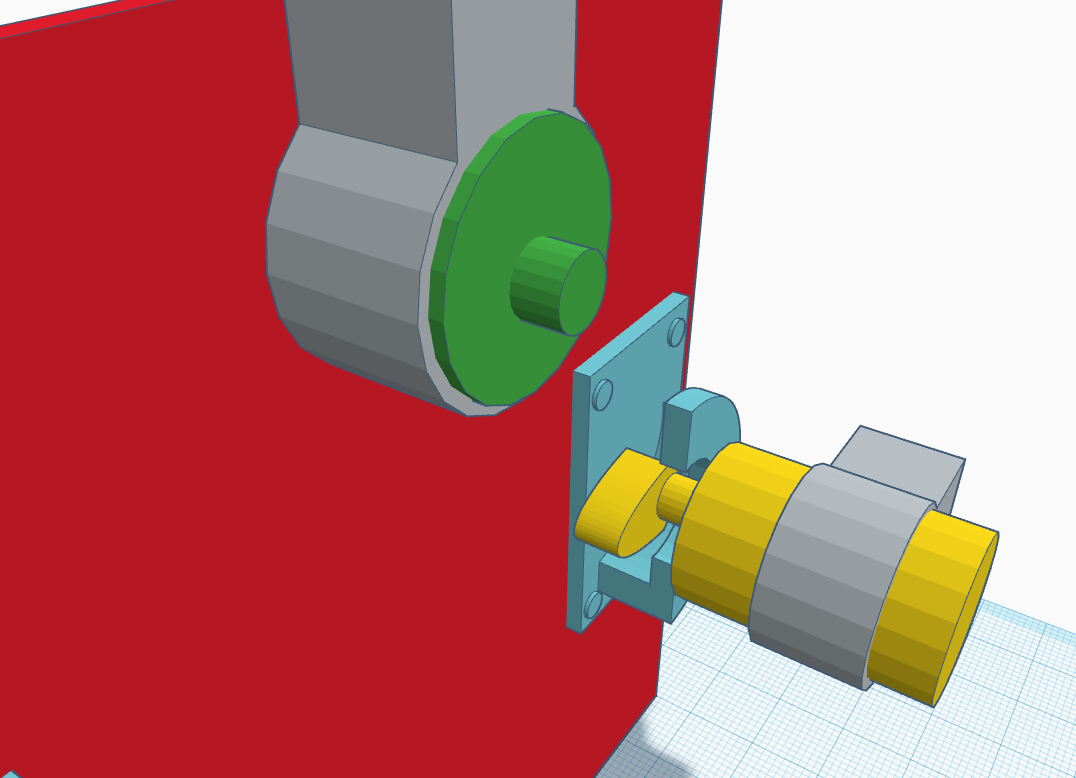
\includegraphics[width=0.85\columnwidth]{Images/OpenLock.png}
    \caption{When the arms are rotated out from the metal plate, the container is unlocked and can manually be opened.}
\end{figure}

\begin{figure}[H]
    \centering
    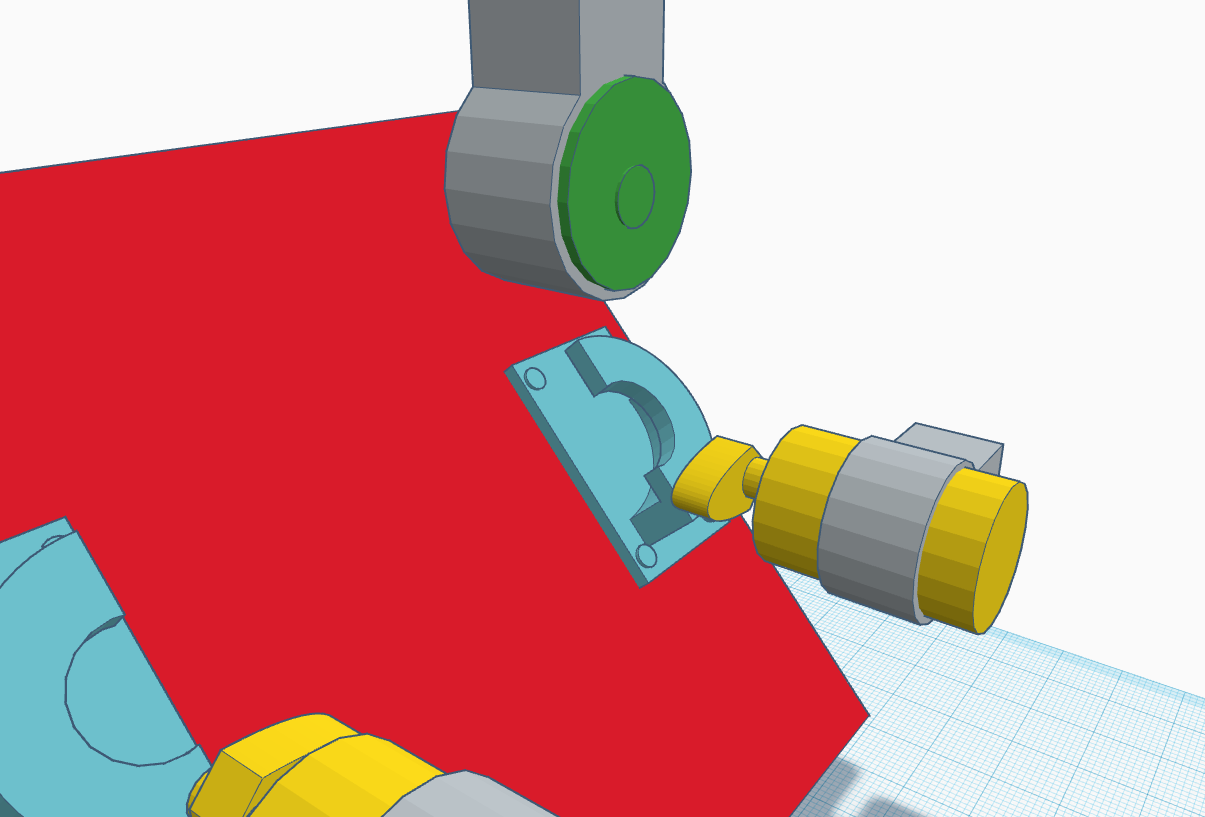
\includegraphics[width=0.85\columnwidth]{Images/OpenContainer.png}
    \caption{The internal solenoid can be used for several effects. For example, when facing the container opening, it can pop the
        door open automatically. If it is facing a wall, it will create a knock sound, or if it does not contact with anything, it can
        make a clicking noise to signal the box is unlocked.}
\end{figure}

\section{Communication Protocols}
As of now, we are trying to decide between two communication protocols that will be used
to control majority of the connections in our room. These two protocols are Wi-Fi and Zigbee,
and each of these have their unique benefits associated with them. A third communication
protocol, bluetooth, is also something that we are thinging of incorporating, however, this
will be more of a secondary communication protocol and will not be the driving force behind
how our components will communicate with each other.

\subsection*{Wi-Fi}
Wi-Fi will act as an incredibly reliable and secure option for our senior project. One of the benefits of Wi-Fi
is that is it so widely supported. There are lots of libraries that would make communication and connection over
Wi-Fi as simple as possible. Plus, the connection range is incredibly good over Wi-Fi, and the data rate is quite high
(around 54 Mbps)~\cite{wifiVsZigbee}. There are two drawbacks to Wi-Fi, however, the first being that it uses a bit more energy than Zigbee
to operate, which may become a problem depending on how many of our components need to operate on a portable energy
source. The second is that there are so many other devices that operate using Wi-Fi, and we may want the privacy that
a connection through Zigbee would provide.

\subsection*{Zigbee}
On the other hand, Zigbee would be an interesting option for a variety of reasons. The most beneficial reason to using
Zigbee would be its topology. Zigbee uses a mesh network topology, which allows each of the network devices to connect with
one another, rather than being dependent upon a central hub to manage the details of the escape room. This would decrease
the number of ``network-hops'' a command would need to traverse, allowing components to tell locks when their puzzle has been
solved. We may end up needing a central hub, so this benefit could nullified, but I digress. Furthermore, Zigbee is much less
widely used than Wi-Fi providing us with a unique experience when trying to get all of our components to communicate
with one another. It also consumes less energy and has a lower data transmission rate than Wi-Fi (maxing out at 250 Kbps),
which could help our wireless components be more energy efficient~\cite{wifiVsZigbee}. These details are yet to be explored,
however, and will need to be more properly considered when we have a more developed plan as to what our escape room is going to require.

\section{Materials Needed}
In order to have a functioning project that we can be proud of, we are going to need a lot of materials.
A list of these materials have been included below
\begin{itemize}
    \item Programmable microcontrollers
    \item Analog clock
    \item Cameras
    \item Small CRT televisions
    \item Chess board and pieces
    \item Audio cassette player
    \item Writable audio cassette tapes
    \item MP3 digital audio controller
    \item Speakers
    \item Motors (To act as lock releases)
    \item Solenoids
    \item LED Display
    \item Adjustable RGB lights
    \item Wireless communication modules
    \item Storage containers
    \item Busts with detachable modules
    \item Turntable podium
\end{itemize}

Various furniture pieces, while not required for functionality, can be used to decorate
the room for an immersive experience. Resistors, capacitors, breadboards, wires, and other
various electronic parts might be required for wiring which can be obtained from the University
of Utah stockroom. Other parts, equipment, or furniture not readily available in the stockroom
will most likely be found sold in the University's surplus store, e-commerce websites like
Amazon, or found in thrift stores and other secondhand locations.

\section{Risk and Mitigation Assessment}
There are various risks that we have identitifed, however, more may present
themselves as we progress through the project. One of the major risks is
the possibility of the items and puzzles in the escape room potentially
breaking which would make the room impossible to complete. A way
to mitigate this risk is to have a manual override that can be activated
if a puzzle is not working as intended. It would also be wise to have
substitute puzzles that can swap in for puzzles that do not work.
\\
\indent There is a risk of evacuation in the case of any emergency that can occur
while players are enjoying the escape room experience. Having cameras
installed in the room will allow the game moderators to keep watch on
the players for safety. On top of this, a way for players to communicate
with the game moderators allow for anybody to exit whenever they like.
A manual override on the lock for the door also means that the
players are never truly locked inside.
\\
\indent Players in the escape room will most likely come across parts of the room
that are not part of the experience and can potentially cause harm if not
handled properly. This may include an outlet on a wall that is installed
in the room beforehand or other electronic components that break easily.
Having signals used for these objects, the risk can be mitigated by letting
players know that they should not be touching or considering that as a
part of a puzzle. This can be done with red tape, where players are instructed
that anything with red tape on it is not part of the escape room and should
not be touched.

\section{Testing}
Different puzzles and modules of the game will be tested before combining
them all into what will become the escape room. Each module will have its
own specifications on what it should do. For example, the chess board puzzle
will have lots of different combinations tested just to make sure that only
the correct one will trigger a signal, which later will be the signal that
allows the players to leave the room. Modules will also be tested on
durability to make sure it is sturdy and not prone to easily breaking.
Players will be instructed to treat every object with care, so hopefully
the modules will not be tested of their strength outside of the testing
environment.
\\
\indent When each module is tested according to their specifications, and works
with small testing programs, then they will be combined into the bigger
room script of the game. From there, testing will be done for the room
as a whole to make sure that players are able to complete it. It may also
be necessary to bring in people unfamiliar with the game to try it out
themselves, that way feedback can be given of whether certain puzzles
need to be harder or easier. For the stretch goal, each possible combination
of puzzles would have to be tested to make sure there are no dead end routes.

\section{Milestones}
For the summer, the milestone set in place will be to obtain all the necessary parts to start work on
the project at the start of the Fall semester. The following tables project what needs to be done by
each team member in the following months:
\begin{table}[ht]
    \centering
    \caption{Milestones for each team member by October.}
    \resizebox{\columnwidth}{!}{
        \begin{tabular}{|l|l|}
            \hline
                          & \multicolumn{1}{c|}{\textbf{\textit{By October}}}                                 \\
            \hline
            \textbf{Nami} & Find a room and plot the layout of where each puzzle and furniture piece will go. \\
            \hline
            \textbf{Kyle} & Build puzzles and other mechanical pieces.                                        \\
            \hline
            \textbf{Jake} & Build connections and communication protocols between puzzles and server.         \\
            \hline
        \end{tabular}
    }
\end{table}

\begin{table}[ht]
    \centering
    \caption{Milestones for each team member by November.}
    \resizebox{\columnwidth}{!}{
        \begin{tabular}{|l|l|}
            \hline
                          & \multicolumn{1}{c|}{\textbf{\textit{By November}}}                                        \\
            \hline
            \textbf{Nami} & Program a timeline of events that the escape room will follow for the players to succeed. \\
            \hline
            \textbf{Kyle} & Create events, experiences, and plots that immerse players into the game world.           \\
            \hline
            \textbf{Jake} & Program and test functionality of individual modules and puzzles.                         \\
            \hline
        \end{tabular}
    }
\end{table}

\begin{table}[ht]
    \centering
    \caption{Milestones for each team member by December.}
    \resizebox{\columnwidth}{!}{
        \begin{tabular}{|l|l|}
            \hline
                          & \multicolumn{1}{c|}{\textbf{\textit{By December}}}                             \\
            \hline
            \textbf{Nami} & Through playtesting, finetune escape room to be fairly solvable in time given. \\
            \hline
            \textbf{Kyle} & Test durability of parts and create substitute puzzles for emergency cases.    \\
            \hline
            \textbf{Jake} & Create new puzzles that can be used for stretch goals.                         \\
            \hline
        \end{tabular}
    }
\end{table}

\section{Resources}
We are going to need a lot of resources in order to complete this senior project.
Our escape room is going to be marginally different from other escape rooms that we have
encountered in the wild due to the autonomous nature of the project. However,
one of the resources that we will be taking advantage of are other escape rooms,
as we would like to do a few before next semester to use them as inspiration for
the puzzles that we will include in our own escape room. For mentors, we plan to interview
people behind escape rooms around the city to see what ideas or technologies go into
designing puzzles within them. Going further into the technical aspect of design, Erik Brunvand
will play a key role into assisting us with any questions and pieces of advice to effectively
create puzzles or desired experiences.

Furthermore, we are going to
be doing a fair amount of research to find documents written by people who have attempted
projects similar to ours. One of which is from a group of Germans who titled their paper
``Teaching Embedded Systems by Constructing an Escape Room''~\cite{germanEscapeRoom}. Their
escape room was constructed as a collection of individual projects completed by various groups
of students, however, the escape room that they were able to create is a great source
of inspiration and we will be on the hunt for other articles such as this.

\section{Prototype Demo and Current Status}
The demo completed for this proposal was the clock that is integral to
the puzzles in the escape room. Players must be expected to manipulate
this clock to activate certain events in the game, along with the clock
moving by itself throughout. Thus, a big analog clock will have controls
tied to it that either moves it forward in time or back in time. The
clock cannot go before 1:00 or past 12:00, and whatever time the clock
is at should be able to be read by a computer.
\\
\indent When in the room, the analog clock will most likely just be a display to an internal
counter that counts on its own based on clock speed. By pressing either a
``forward'' or ``reverse'' button, the counter will increment or decrement
and update the display on the clock alongside transferring the value to
a computer. This will make the time easily stored and tracked which will
help towards scripting certain events in the escape room. For the prototype demonstration,
the clock just used a standard DC motor, STM32F0 microcontroller, and some buttons
to make the hands move at a rate of about one clock hour per real minute when idle, and
maximum speed forward and backward when the appropriate button was pressed. To finish out
the clock to function within the escape room itself, endstop switches will be placed at
the 1:00 and 12:00 hour times, as well as an encoder and counter to track the actual time
of the game clock. These ``home'' positions for the hour hands will be tracked with 3-pin
end stop switches similar to the ones found on delta 3D printers/ The light pressure sensativity
and metal switch arm will make them easy to install on the clock in a safe manner.
\\
\indent Aside from our prototype components, we have also collected many
parts that will be used in the final project. We will be making extensive
use of Arduino controllers, as well as raspberry pi computers for room control.
We have collected the audio cassette player with 8 blank tapes, a remote MP3
controller, 3D printing filament, some CRT displays and cables, and several
electronic components that will be used to ``hack'' existing hardware for the
purposes of this escape room (such as hijacking audio signals from the cassette
player).

%   ********************************************************************************************************
%   ********************* CONCLUSION TO BE COMPLETED TOGETHER **********************************************
%   ********************************************************************************************************
\section{Conclusion}
In conclusion, we are confident that this project will help us grow and become more capable
engineers in the future. We are going to learn more about how to deal with lots of interconnected
micro-systems, how to create a compelling and immersive story, how to properly document and track
our work, and how to work together as a team on a long-term development project. All of these things
are incredibly valuable to prospective employers, and we are excited to leave college as prepared
as possible to enter the workforce. Furthermore, this is a project that we are all incredibly excited
about, which will help us produce something that we can be proud of by the end of next semester!

\begin{thebibliography}{00}

    \bibitem{wikipediaEscapeRoom} “Escape room,” Wikipedia, 10-Feb-2023. [Online]. Available: \url{https://en.wikipedia.org/wiki/Escape_room}. [Accessed: 24-Mar-2023].
    \bibitem{whatIsAnEscapeRoom} A. Ascalon, “Escape rooms: Everything you need to know (2022),” Escape Rooms | Everything You Need To Know (2022), 01-Dec-2022. [Online]. Available:  \url{https://theescapegame.com/blog/what-is-an-escape-room/}. [Accessed: 24-Mar-2023].
    \bibitem{germanEscapeRoom} M. Pfeifer, B. Völker, S. Böttcher, S. Köhler, and P. M. Scholl, “Teaching embedded systems by constructing an escape room,” Proceedings of the 52nd ACM Technical Symposium on Computer Science Education, 2021.
    \bibitem{wifiVsZigbee} B. Priya, “What are the differences between Zigbee and Wi-Fi,” Tutorials Point, 17-Mar-2022. [Online]. Available: \url{https://www.tutorialspoint.com/what-are-the-differences-between-zigbee-and-wi-fi}. [Accessed: 03-May-2023].

\end{thebibliography}




\end{document}
